\chapter{Inverse Functions and Limits}

\section{Inverse Functions and One-to-One Functions}

In many situations, a function describes a process that sends an input \(x\) to an output \(y=f(x)\). We are often interested in reversing this process and recovering the original input from the output. This leads to the ideas of one-to-one functions and inverse functions.

\subsection{One-to-One Functions}

A function can have an inverse only when each output comes from exactly one input. This motivates the following definition.

\begin{definition}
Let \(f\) be a function with domain \(A\). We say that \(f\) is \emph{one-to-one} if
\[
f(x_1)\ne f(x_2)
\qquad \text{whenever } x_1\ne x_2.
\]
Equivalently, \(f\) is one-to-one if
\[
f(x_1)=f(x_2) \implies x_1=x_2.
\]
\end{definition}

\begin{example}
Let's look at some everyday scenarios. Consider the functions mapping a group of students to their personal details:
\[
f(\text{student})=\text{Student ID number}
\]
and
\[
g(\text{student})=\text{Blood type}.
\]
Determine which of these real-world functions are one-to-one.
\end{example}

\begin{solution}
The function \(f\) is one-to-one because every student gets a unique ID number. Distinct inputs always give distinct outputs, so each ID number corresponds to exactly one student.

The function \(g\) is not one-to-one because different students can share the same blood type. For instance, if Alice and Bob are both Type O, then
\[
g(\text{Alice})=\text{Type O}
\qquad \text{and} \qquad
g(\text{Bob})=\text{Type O}.
\]
Since two different inputs produce the same output, \(g\) is not one-to-one.
\end{solution}

Now let us consider some mathematical examples.

\begin{example}
Consider the functions
\[
f(x)=x, \qquad 0\le x\le 1,
\]
and
\[
g(x)=x^2, \qquad -1\le x\le 1.
\]
Determine which of these functions are one-to-one.
\end{example}

\begin{solution}
The function \(f(x)=x\) is one-to-one on \([0,1]\) because distinct inputs always produce distinct outputs.

The function \(g(x)=x^2\) is not one-to-one on \([-1,1]\) because
\[
g\left(\frac12\right)=\left(\frac12\right)^2=\frac14
\qquad \text{and} \qquad
g\left(-\frac12\right)=\left(-\frac12\right)^2=\frac14.
\]
Thus two different inputs produce the same output, so \(g\) is not one-to-one.
\end{solution}

The previous example shows that not every function has an inverse. For \(g(x)=x^2\) on \([-1,1]\), the value \(\frac14\) comes from both \(\frac12\) and \(-\frac12\). Therefore there is no unique value that can be assigned to \(g^{-1}\!\left(\frac14\right)\).

\begin{theorem}[Horizontal Line Test]
A function is one-to-one if and only if no horizontal line intersects its graph more than once.
\end{theorem}


A horizontal line has equation $y=c$, so it represents a fixed output value $c$.
If the line $y=c$ intersects the graph of $f$ at least two distinct points $(x_1,c)$ and $(x_2,c)$ with $x_1\neq x_2$, then
\[
f(x_1)=c=f(x_2).
\]
Thus two different inputs produce the same output, so $f$ is not one-to-one.
Conversely, if every horizontal line intersects the graph at most once, then no output value corresponds to more than one input, and hence $f$ is one-to-one.

\begin{figure}[ht]
\centering
\begin{minipage}{0.46\textwidth}
\centering
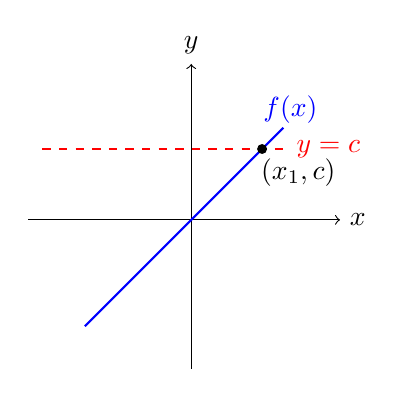
\begin{tikzpicture}[scale=0.9]
\draw[->] (-2.3,0) -- (2.1,0) node[right] {$x$};
\draw[->] (0,-2.1) -- (0,2.2) node[above] {$y$};
\draw[blue, thick] (-1.5,-1.5) -- (1.3,1.3);
\draw[red, dashed] (-2.1,1) -- (1.3,1);
\fill (1,1) circle (2pt);
\node[blue] at (1.4,1.55) {$f(x)$};
\node[below right] at (0.85,1) {$(x_1,c)$};
\node[red, right] at (1.35,1) {$y=c$};
\end{tikzpicture}

\vspace{0.4em}
One-to-one function\\
Intersects at most once.
\end{minipage}
\hfill
\begin{minipage}{0.46\textwidth}
\centering
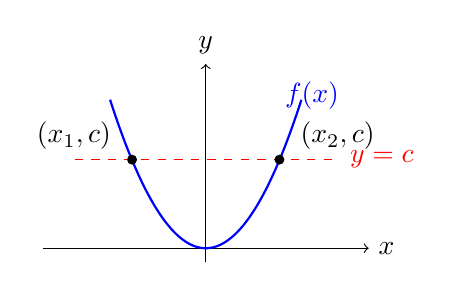
\begin{tikzpicture}[scale=0.9]
\draw[->] (-2.3,0) -- (2.3,0) node[right] {$x$};
\draw[->] (0,-0.2) -- (0,2.6) node[above] {$y$};
\draw[blue, thick, domain=-1.35:1.35, samples=100] plot (\x,{1.15*\x*\x});
\draw[red, dashed] (-1.85,1.25) -- (1.85,1.25);
\fill (-1.04,1.25) circle (2pt);
\fill (1.04,1.25) circle (2pt);
\node[blue] at (1.5,2.15) {$f(x)$};
\node[above left] at (-1.2,1.25) {$(x_1,c)$};
\node[above right] at (1.2,1.25) {$(x_2,c)$};
\node[red, right] at (1.9,1.25) {$y=c$};
\end{tikzpicture}

\vspace{0.4em}
Not one-to-one\\
Intersects more than once.
\end{minipage}
\caption{Geometric interpretation of the horizontal line test.}
\end{figure}

\subsection{Inverse Functions}

Suppose that \(f\) is a one-to-one function. If \(f\) maps \(x\) to \(y\), then its inverse maps \(y\) back to \(x\).

\begin{definition}
Let \(f\) be a one-to-one function with domain \(A\) and range \(B\). Then the \emph{inverse function} of \(f\), denoted by \(f^{-1}\), has domain \(B\) and range \(A\), and is defined by
\[
f^{-1}(y)=x
\quad \Longleftrightarrow \quad
f(x)=y,
\qquad y\in B.
\]
\end{definition}

\begin{remark}
When we focus on the inverse function, it is common to use \(x\) as the independent variable. In that case we may write
\[
f^{-1}(x)=y
\quad \Longleftrightarrow \quad
f(y)=x.
\]
\end{remark}

\begin{example}
Find the inverse of each function.
\begin{enumerate}
    \item \(f(x)=x\)
    \item \(g(x)=x^3\)
\end{enumerate}
\end{example}

\begin{solution}
\leavevmode
\begin{enumerate}
    \item  Since \(f(x)=x\) leaves every input unchanged, its inverse is also
    \[
    f^{-1}(x)=x.
    \]

    \item Let
    \[
    y=x^3.
    \]
    Solving for \(x\), we obtain
    \[
    x=\sqrt[3]{y}.
    \]
    Interchanging \(x\) and \(y\), we get
    \[
    g^{-1}(x)=\sqrt[3]{x}.
    \]
\end{enumerate}
\end{solution}

\begin{proposition}
Let \(f\) be a one-to-one function with domain \(A\) and range \(B\). Then
\[
f^{-1}(f(x))=x
\qquad \text{for every } x\in A,
\]
and
\[
f(f^{-1}(x))=x
\qquad \text{for every } x\in B.
\]

\begin{figure}[htbp]
    \centering
    \begin{tikzpicture}[
        transform shape,
        >=Stealth,
        every node/.style={font=\small},
        lab/.style={midway, fill=white, inner sep=1pt},
        mainnode/.style={text=blue!50!black},
        fwd/.style={->, very thick, draw=blue!50!blue},
        bwd/.style={->, very thick, draw=red!70!blue}
    ]

    % left diagram
    \node[mainnode] (xA) at (0,0) {$x\in A$};
    \node[mainnode] (fxB) at (4.8,0) {$f(x)\in B$};

    \draw[fwd, bend left=10] (xA) to node[lab, above, text=blue!40!black] {$f$} (fxB);
    \draw[bwd, bend left=10] (fxB) to node[lab, below, text=red!70!black] {$f^{-1}$} (xA);

    \node[text=blue!60!black] at (2.4,-1) {$f^{-1}(f(x))=x$};

    % right diagram
    \node[mainnode] (xB) at (8.2,0) {$x\in B$};
    \node[mainnode] (finvxA) at (13,0) {$f^{-1}(x)\in A$};

    \draw[bwd, bend left=10] (xB) to node[lab, above, text=red!70!black] {$f^{-1}$} (finvxA);
    \draw[fwd, bend left=10] (finvxA) to node[lab, below, text=blue!40!black] {$f$} (xB);

    \node[text=blue!60!black] at (10.6,-1) {$f\bigl(f^{-1}(x)\bigr)=x$};

    \end{tikzpicture}
    \caption{one-to-one function and its inverse.}
    \label{fig:inverse-composition}
\end{figure}

\end{proposition}

\newpage

\subsection{Finding the Inverse of a Function}

When \(f\) is one-to-one, the following procedure is often useful for finding \(f^{-1}\).

\begin{remark}
To find the inverse of a one-to-one function \(f\), we may proceed as follows:
\begin{enumerate}
    \item Write
    \[
    y=f(x).
    \]
    \item Solve this equation for \(x\) in terms of \(y\).
    \item Interchange \(x\) and \(y\). The resulting equation gives \(f^{-1}(x)\).
\end{enumerate}
\end{remark}

\begin{example}
Find the inverse of
\[
f(x)=x^3+2.
\]
\end{example}

\begin{solution}
Let
\[
y=x^3+2.
\]
Then
\[
x^3=y-2,
\]
so
\[
x=\sqrt[3]{\,y-2\,}.
\]
Interchanging \(x\) and \(y\), we obtain
\[
f^{-1}(x)=\sqrt[3]{\,x-2\,}.
\]
We check this by composition:
\[
f\bigl(f^{-1}(x)\bigr)
=
\left(\sqrt[3]{\,x-2\,}\right)^3+2
=
x-2+2
=
x.
\]
Thus the inverse is correct.
\end{solution}

 %-----------------------------------------------------
 %反三角函數
 %-----------------------------------------------------

\section{Inverse Trigonometric Functions}

The trigonometric functions are not one-to-one on all of \(\mathbb{R}\), so they do not have inverse functions on their full domains. To define inverse trigonometric functions, we restrict the domains of the trigonometric functions so that they become one-to-one.

Consider the sine function on all of \(\mathbb{R}\). As shown in Figure~\ref{fig:sine-not-one-to-one}, a horizontal line can intersect the graph of \(y=\sin x\) more than once. Therefore \(\sin x\) is not one-to-one on \(\mathbb{R}\), and so it does not have an inverse function on its full domain.

\begin{figure}[ht]
\centering
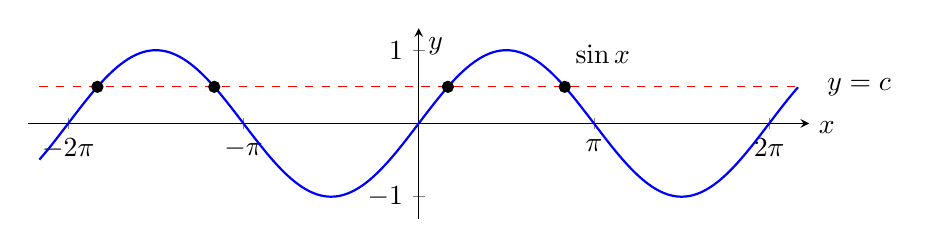
\begin{tikzpicture}
\begin{axis}[
width=11.5cm,
height=4cm,
axis lines=middle,
xmin=-7,
xmax=7,
ymin=-1.3,
ymax=1.3,
xtick={-6.283185307,-3.141592654,0,3.141592654,6.283185307},
xticklabels={\(-2\pi\),\(-\pi\),\(0\),\(\pi\),\(2\pi\)},
ytick={-1,1},
yticklabels={\(-1\),\(1\)},
xlabel={\(x\)},
xlabel style={at={(axis description cs:1.0,0.48)}, anchor=west},
ylabel={\(y\)},
samples=300,
clip=false
]
\addplot[thick, blue, domain=-6.8:6.8] {sin(deg(x))};
\addplot[dashed, red] coordinates {(-6.8,0.5) (6.8,0.5)};
\addplot[only marks, mark=*, mark size=2pt] coordinates {
(0.523598776,0.5)    % pi/6
(2.617993878,0.5)    % 5pi/6
(-3.665191429,0.5)   % -7pi/6
(-5.759586531,0.5)   % -11pi/6
};
\node at (axis cs:3.3,0.95) {\(\sin x\)};
\node[right] at (axis cs:7.15,0.5) {\(y=c\)};
\end{axis}
\end{tikzpicture}
\caption{The sine function on \(\mathbb{R}\) is not one-to-one.}
\label{fig:sine-not-one-to-one}
\end{figure}

\subsection{The inverse sine function}

To define the inverse sine function, we restrict \(\sin x\) to the interval
\[
-\frac{\pi}{2}\le x\le \frac{\pi}{2}.
\]
On this interval, \(\sin x\) is one-to-one, and every value in the range \([-1,1]\) is attained. The restricted branch is shown in Figure~\ref{fig:restricted-sine}.

\begin{figure}[ht]
\centering
\begin{tikzpicture}
\begin{axis}[
width=8.5cm,
height=5.6cm,
axis lines=middle,
xmin=-1.9,
xmax=1.9,
ymin=-1.2,
ymax=1.2,
xtick={-1.570796327,1.570796327},
xticklabels={\(-\frac{\pi}{2}\),\(\frac{\pi}{2}\)},
ytick={-1,1},
yticklabels={\(-1\),\(1\)},
xlabel={\(x\)},
ylabel={\(y\)},
samples=200,
clip=false
]
\addplot[thick,blue, domain=-1.570796327:1.570796327] {sin(deg(x))};
\node at (axis cs:0.95,1.1) {\(\sin x\)};
\end{axis}
\end{tikzpicture}
\caption{Restricted branch of the sine function used to define \(\arcsin x\).}
\label{fig:restricted-sine}
\end{figure}

\begin{definition}
The \emph{inverse sine function}, denoted by \(\arcsin x\), is defined by
\[
\arcsin x=y
\quad \Longleftrightarrow \quad
\sin y=x
\quad \text{and} \quad
-\frac{\pi}{2}\le y\le \frac{\pi}{2}.
\]
\end{definition}

\begin{remark}
The domain of \(\arcsin x\) is \([-1,1]\), and its range is
\[
\left[-\frac{\pi}{2},\frac{\pi}{2}\right].
\]
Also,
\[
\arcsin(\sin x)=x,
\qquad -\frac{\pi}{2}\le x\le \frac{\pi}{2},
\]
and
\[
\sin(\arcsin x)=x,
\qquad -1\le x\le 1.
\]
\end{remark}

\begin{example}
Evaluate the following expressions.
\begin{enumerate}
    \item \(\arcsin\left(\dfrac{1}{2}\right)\)
    \item \(\tan\left(\arcsin\left(\dfrac{1}{3}\right)\right)\)
\end{enumerate}
\end{example}

\begin{solution}
\leavevmode
\begin{enumerate}
    \item We seek the number \(y\) in the interval
    \[
    -\frac{\pi}{2}\le y\le \frac{\pi}{2}
    \]
    such that
    \[
    \sin y=\frac{1}{2}.
    \]
    Since
    \[
    \sin\left(\frac{\pi}{6}\right)=\frac{1}{2},
    \]
    it follows that
    \[
    \arcsin\left(\frac{1}{2}\right)=\frac{\pi}{6}.
    \]

    \item Let
    \[
    \theta=\arcsin\left(\frac{1}{3}\right).
    \]
    Then
    \[
    \sin\theta=\frac{1}{3},
    \qquad
    -\frac{\pi}{2}\le \theta\le \frac{\pi}{2}.
    \]
    Since \(\sin\theta>0\), we take \(\theta\) in the first quadrant. A right triangle corresponding to this relation is shown in Figure~\ref{fig:tan-arcsin-triangle}.

    \begin{figure}[ht]
    \centering
    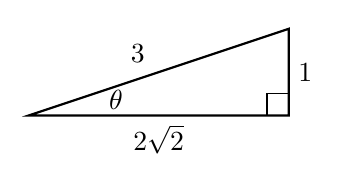
\begin{tikzpicture}[scale=1.1]
    \coordinate (A) at (0,0);
    \coordinate (B) at (3,0);
    \coordinate (C) at (3,1);
    \draw[thick] (A) -- (B) -- (C) -- cycle;
    \draw (2.75,0) -- (2.75,0.25) -- (3,0.25);
    \node[left] at (1.2,0.18) {\(\theta\)};
    \node[below] at (1.5,0) {\(2\sqrt{2}\)};
    \node[right] at (3,0.5) {\(1\)};
    \node[above left] at (1.45,0.5) {\(3\)};
    \end{tikzpicture}
    \caption{A right-triangle interpretation of \(\tan(\arcsin(1/3))\).}
    \label{fig:tan-arcsin-triangle}
    \end{figure}

    By the Pythagorean Theorem, the adjacent side is
    \[
    \sqrt{3^{2}-1^{2}}=\sqrt{8}=2\sqrt{2}.
    \]
    Therefore,
    \[
    \tan\theta=\frac{1}{2\sqrt{2}}.
    \]
    Hence
    \[
    \tan\left(\arcsin\left(\frac{1}{3}\right)\right)=\frac{1}{2\sqrt{2}}.
    \]
\end{enumerate}
\end{solution}

\subsection{The inverse cosine function}

The cosine function becomes one-to-one when its domain is restricted to
\[
0\le x\le \pi.
\]
The restricted branch is shown in Figure~\ref{fig:restricted-cosine}.

\begin{figure}[ht]
\centering
\begin{tikzpicture}
\begin{axis}[
width=8.5cm,
height=5.6cm,
axis lines=middle,
xmin=-0.3,
xmax=3.5,
ymin=-1.3,
ymax=1.5,
xtick={0,3.141592654},
xticklabels={\(0\),\(\pi\)},
ytick={-1,1},
yticklabels={\(-1\),\(1\)},
xlabel={\(x\)},
ylabel={\(y\)},
samples=200,
clip=false
]
\addplot[thick,blue, domain=0:3.141592654] {cos(deg(x))};
\node at (axis cs:1.2,0.72) {\(\cos x\)};
\end{axis}
\end{tikzpicture}
\caption{Restricted branch of the cosine function used to define \(\arccos x\).}
\label{fig:restricted-cosine}
\end{figure}

\begin{definition}
The \emph{inverse cosine function}, denoted by \(\arccos x\), is defined by
\[
\arccos x=y
\quad \Longleftrightarrow \quad
\cos y=x
\quad \text{and} \quad
0\le y\le \pi.
\]
\end{definition}

\begin{remark}
The domain of \(\arccos x\) is \([-1,1]\), and its range is
\[
[0,\pi].
\]
Also,
\[
\arccos(\cos x)=x,
\qquad 0\le x\le \pi,
\]
and
\[
\cos(\arccos x)=x,
\qquad -1\le x\le 1.
\]
\end{remark}

\subsection{The inverse tangent function}

The tangent function becomes one-to-one when its domain is restricted to
\[
-\frac{\pi}{2}<x<\frac{\pi}{2}.
\]
The restricted branch is shown in Figure~\ref{fig:restricted-tangent}.

\begin{figure}[ht]
\centering
\begin{tikzpicture}
\begin{axis}[
width=8.5cm,
height=8.5cm,
axis lines=middle,
xmin=-1.9,
xmax=1.9,
ymin=-5,
ymax=5,
xtick={-1.570796327,1.570796327},
xticklabels={\(-\frac{\pi}{2}\),\(\frac{\pi}{2}\)},
ytick=\empty,
xlabel={\(x\)},
ylabel={\(y\)},
samples=200,
clip=false
]
\addplot[dashed] coordinates {(-1.570796327,-5) (-1.570796327,5)};
\addplot[dashed] coordinates {(1.570796327,-5) (1.570796327,5)};
\addplot[thick,blue, domain=-1.35:1.35] {tan(deg(x))};
\node at (axis cs:0.65,1.55) {\(\tan x\)};
\end{axis}
\end{tikzpicture}
\caption{Restricted branch of the tangent function used to define \(\arctan x\).}
\label{fig:restricted-tangent}
\end{figure}

\begin{definition}
The \emph{inverse tangent function}, denoted by \(\arctan x\), is defined by
\[
\arctan x=y
\quad \Longleftrightarrow \quad
\tan y=x
\quad \text{and} \quad
-\frac{\pi}{2}<y<\frac{\pi}{2}.
\]
\end{definition}

\begin{remark}
The domain of \(\arctan x\) is \(\mathbb{R}\), and its range is
\[
\left(-\frac{\pi}{2},\frac{\pi}{2}\right).
\]
Also,
\[
\arctan(\tan x)=x,
\qquad -\frac{\pi}{2}<x<\frac{\pi}{2},
\]
and
\[
\tan(\arctan x)=x,
\qquad x\in\mathbb{R}.
\]
\end{remark}

\begin{example}
Simplify \(\cos(\arctan x)\).
\end{example}

\begin{solution}
Let
\[
y=\arctan x.
\]
Then
\[
\tan y=x,
\qquad
-\frac{\pi}{2}<y<\frac{\pi}{2}.
\]
We want to find \(\cos y\). Using the identity
\[
1+\tan^{2}y=\sec^{2}y,
\]
we obtain
\[
\sec^{2}y=1+x^{2}.
\]
Since
\[
-\frac{\pi}{2}<y<\frac{\pi}{2},
\]
we have \(\cos y>0\), and hence \(\sec y>0\). Therefore,
\[
\sec y=\sqrt{1+x^{2}}.
\]
It follows that
\[
\cos y=\frac{1}{\sec y}=\frac{1}{\sqrt{1+x^{2}}}.
\]
Thus
\[
\cos(\arctan x)=\frac{1}{\sqrt{1+x^{2}}}.
\]
\end{solution}

\subsection{The remaining inverse trigonometric functions}

The remaining inverse trigonometric functions are listed below. They are not used as frequently.
\[
y=\csc^{-1}x \quad (|x|\ge 1)
\quad \Longleftrightarrow \quad
\csc y=x,
\qquad
y\in \left(0,\frac{\pi}{2}\right]\cup\left(\pi,\frac{3\pi}{2}\right]
\]
\[
y=\sec^{-1}x \quad (|x|\ge 1)
\quad \Longleftrightarrow \quad
\sec y=x,
\qquad
y\in \left[0,\frac{\pi}{2}\right)\cup\left[\pi,\frac{3\pi}{2}\right)
\]
\[
y=\cot^{-1}x \quad (x\in\mathbb{R})
\quad \Longleftrightarrow \quad
\cot y=x,
\qquad
y\in (0,\pi)
\]

\begin{remark}
For \(\sec^{-1}x\), we also can choose \(y\in \left[0,\frac{\pi}{2}\right)\cup\left(\frac{\pi}{2},\pi\right]\). The reason for the choice \(y\in \left[0,\frac{\pi}{2}\right)\cup\left[\pi,\frac{3\pi}{2}\right)\) is that the differentiation formulas are simpler.
\end{remark}